\subsubsection{Policy maker scenarios}
\subsubsection*{Scenario 5}
Gurleen, a Telengana’s Policy maker, needs to visualize data about agricultural harvest quality. Gurleen connects at Dream’s site and lands at the home page. She clicks a button in the top right of the screen with the words “Sign In”. Gurleen is already registered to the service, so she authenticates digiting her email and password and accesses to her reserved area. From this screen she accesses the Deviance section and from that point she can visualize a ranking list, established by Dream project’s service, of the different areas. At this point, she identifies the areas with the best score and publishes a document, publicly visible, where she asks to the farmers to present a report about their cultivation techniques, that will be published in the forum.

\subsubsection*{Scenario 6}
Digamber, another Policy maker from the same area of Gurleen, checks his email and notice a notification from Dream about a new publication in a discussion that he has created. Clicking on the link from the email he opens the correspondent forum discussion. Once he has read Gurleeen’s replies he notice that he can’t answer because he isn’t logged in. So he clicks the “Sign In” button in the top right and he fills the fields with his username and password to authenticate. In this way he can write his replies and publish it in the discussion.

\subsubsection*{Scenario 7}
Bipin is a Telengana’s Policy maker. His boss asked him to check the efficiency of agricultural production in the district of Medak. Bipin goes to the Dream site home page and since is the first time he’s assigned this job he has firstly to register to the portal. He clicks on the “Registration” button on the top right and inserts his data in the following page. He’s asked for his personal code (Policy maker ID) which identifies him as Policy maker and eventually he confirms data insertion. A mail is send to the email address used during the registration with a confirmation link that once clicked consent to activate the new account. Bipin clicks on it and land on a confirmation page.

\subsubsection*{Scenario 8}
Akash is a Policy maker of Telengana and needs to manage the forum of the Dream’s site. Akash then connects to the home page of the Dream’s site and since he is already logged in, he can go directly on the forum page, by clicking a button present on the home page. When he reaches the forum, Akash clicks on the “Moderator area”, then he selects the pending list option and from that moment he can see a pending list with all the posts that required approval before being published in the forum. Akash decides to open the first post, examine it and then he approves it to be published; after the confirmation by Akash, the system automatically publishes the post in the forum and sends a notification to the author of the post.

\subsubsection*{Scenario 9}
Parag is a Policy maker already registered in Dream’s site. Today he needs to recalculate the Deviance according to certain parameters, told by his boss. So since he is already logged in, he can go directly to his reserved area, by clicking a button present on the home page. After doing that he selects the Deviance section and from that moment he can see the actual ranking list, calculated by default by the system, and a list of parameters that he can select in order to recalculate a custom Deviance. He selects on three different parameters and then clicks on recalculate. The system recalculates the Deviance and then reloads the contents, showing the new custom ranking list.

\subsubsection*{Use case diagram}
\begin{figure}[h!]
        \centering
        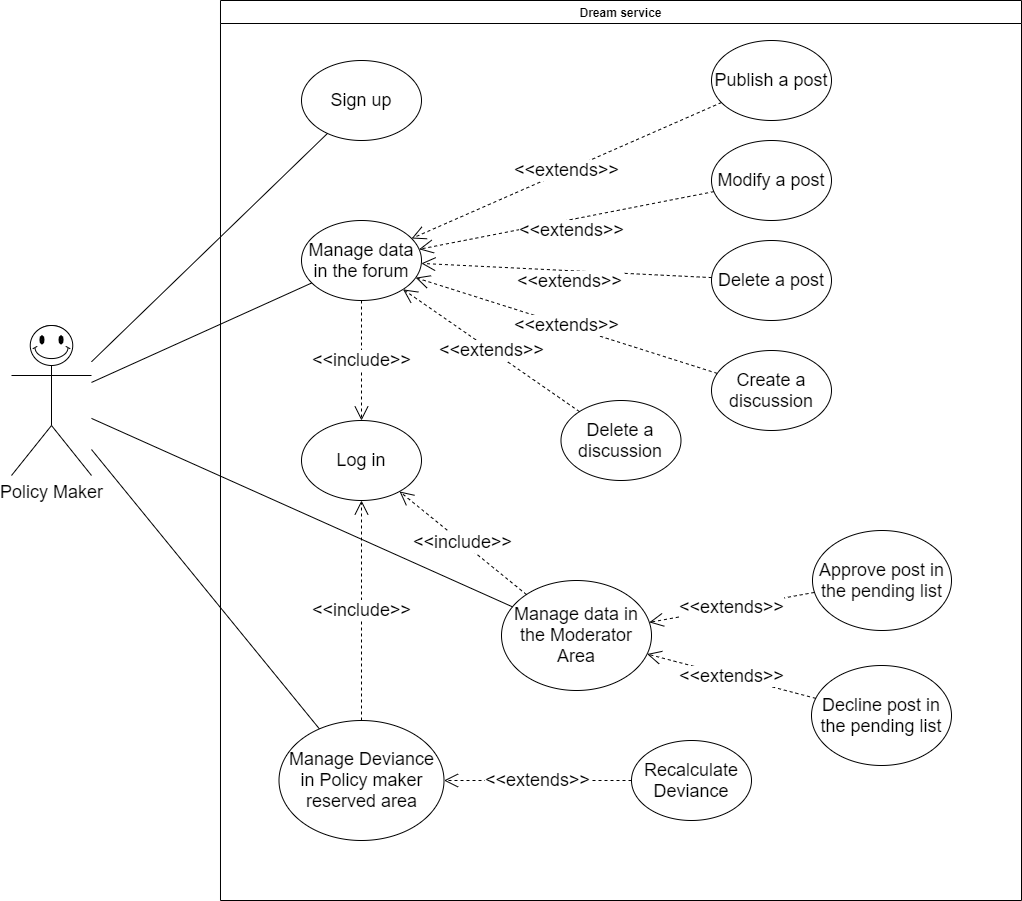
\includegraphics[scale=0.35]{images/use_cases_diagram/policymaker_use_case.png}
        \caption{Use case diagram}
        \label{fig:policy_maker_use_case}
    \end{figure}
 \newpage
\subsubsection*{Use case tables}

\begin{longtable}{p{.25\textwidth} | p{.75\textwidth}}
\caption{Sign Up Policy maker}
        \label{tab:signup_policy_maker}\\
        \hline
        \textbf{ID} & 9\\
        \hline
        \textbf{Name}  &  Sign up Policy maker\\
        \hline
        \textbf{Actor}  &  Policy maker\\
        \hline
        \textbf{Entry condition}  &  Policy maker has reached the site\\
        \hline
        \textbf{Input}  & Personal data, Policy maker ID, email and password to use for the registration\\ 
        \hline
        \textbf{Events flow} & 
        \begin{itemize}
                \item The site displays the “Sign Up” button on the top right of the screen
                \item Policy maker clicks on “Sign Up”
                \item The site displays a new page containing blank fields where user has to insert his data: name, surname, Policy maker ID, date of birth, area of residence, email and password
                \item Policy maker inserts the mandatory data and the Policy maker ID
                \item Policy maker confirms by clicking the confirmation button
                \item The page shows a message inviting Policy maker to visit his email address in order to conclude the registration
                \item Policy maker opens his inbox, find the email from Dream and clicks on confirmation link
                \item The site displays a confirmation message of successful registration
                 \end{itemize}
                 \\
        \hline
        \textbf{Exit condition} & Policy maker registration has been successful: the inserted data are stored in the database of the system. Now Policy maker can login using his credentials and post in the forum\\
        \hline
        \textbf{Output} & Registration data are stored in the database of Dream site.\\
        \hline
        \textbf{Exceptions} & 
        \begin{itemize}
            \item Policy maker inserts non valid data (wrong date format or nonexistent area). The application displays an error message telling the Policy maker that he must check the data inserted and correct the invalid ones. 
            \item Policy maker inserts an email which is already stored in the database. So, after user inserts his data and clicks on confirm, the application displays an error message telling User that he’s already registered to the service and invites him to login with that email
            \item Policy maker inserts a non valid ID
            \item Policy maker inserts data non corresponding to the ID
        \end{itemize}\\
        \hline
       
        
    \end{longtable}

\begin{figure}[h!]
        \centering
        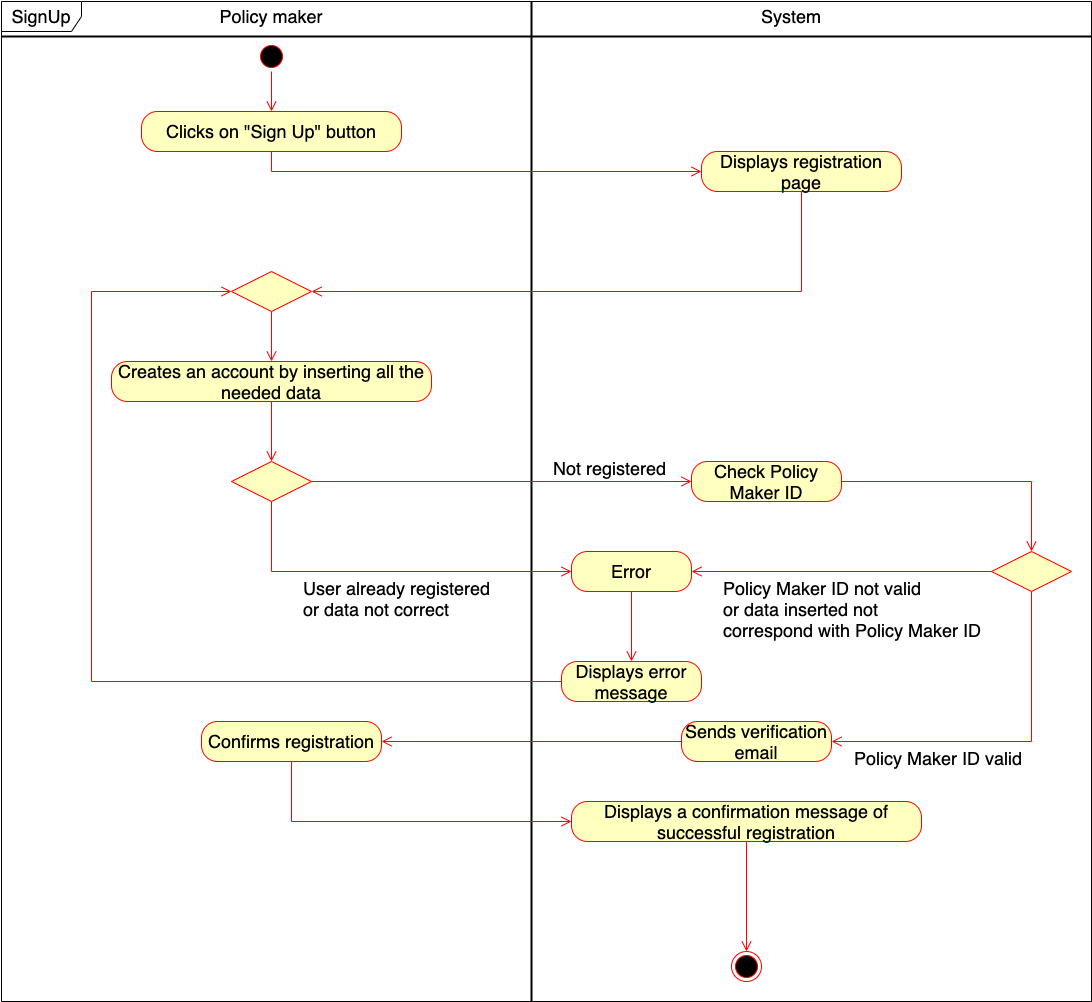
\includegraphics[scale=0.30]{images/use_cases_diagram/policymaker_sign_up.png}
        \caption{Sign Up Policy maker}
        \label{fig:policymaker_sign_up}
    \end{figure}
\FloatBarrier

\begin{longtable}{p{.25\textwidth} | p{.75\textwidth}}
\caption{Login Policy maker}
        \label{tab:login_policy_maker}\\
        \hline
        \textbf{ID} & 10\\
        \hline
        \textbf{Name}  &  Login Policy maker \\
        \hline
        \textbf{Actor}  &  Policy maker\\
        \hline
        \textbf{Entry condition}  &  
        \begin{itemize}
                \item Policy maker has reached the site
                \item Policy maker is already registered to the platform
         \end{itemize}\\
        \hline
        \textbf{Input}  & Policy maker email and password associated to a successful registration\\ 
        \hline
        \textbf{Events flow} & 
        \begin{itemize}
                \item The site displays the “Sign in” button on the top right of the screen
                \item Policy maker clicks on “Sign In"
                \item The system displays the login page
                \item Policy maker fills the username (email) and password fields using the credential inserted during the registration
                \item System checks the validity of the credentials inserted
                \item The system displays the precedent page or, if unavailable, the home page of the Policy maker dashboard
                 \end{itemize}
                 \\
        \hline
        \textbf{Exit condition} & Policy maker is logged in\\
        \hline
        \textbf{Exceptions} & Policy maker inserts wrong credentials and clicks on login button. The system shows an error message inviting the Policy maker to check the credentials before trying again to login\\
        \hline
       
        
    \end{longtable}
    
    \begin{figure}[h!]
        \centering
        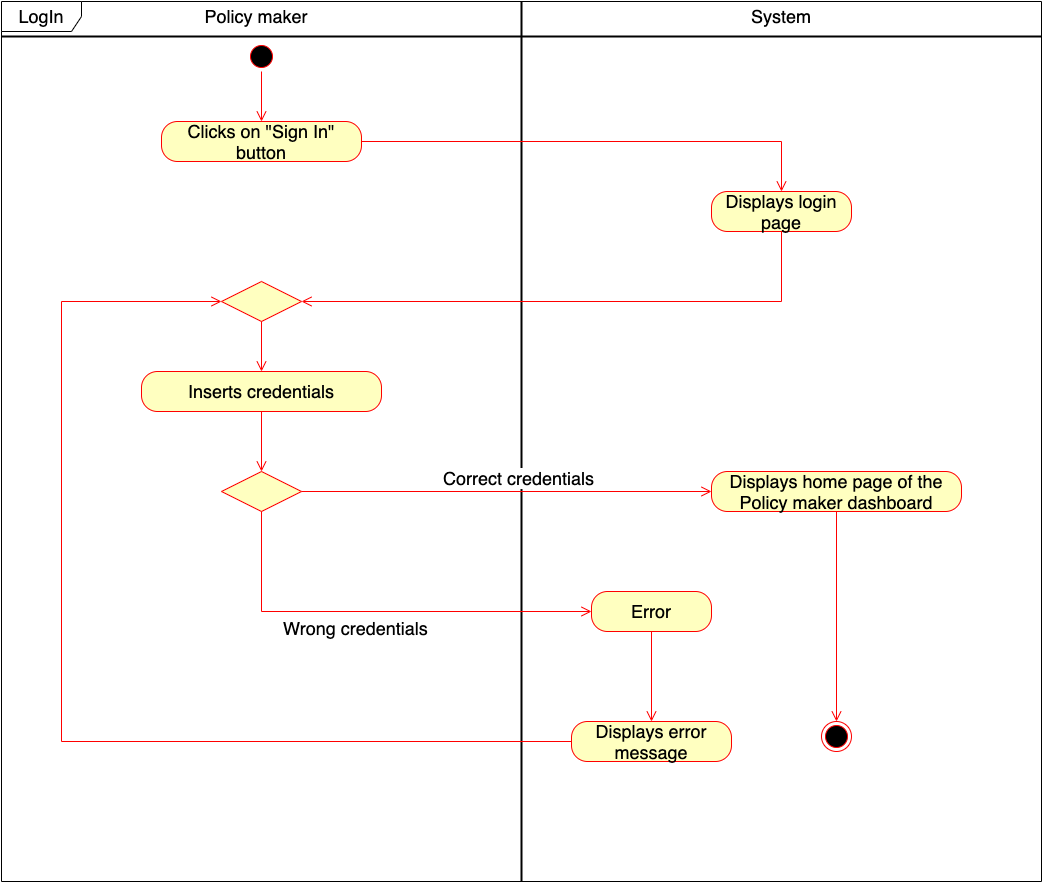
\includegraphics[scale=0.35]{images/use_cases_diagram/policymaker_login.png}
        \caption{Login Policy maker}
        \label{fig:policymaker_login}
    \end{figure}
    \FloatBarrier
    
    \begin{longtable}{p{.25\textwidth} | p{.75\textwidth}}
    \caption{Publish a post by Policy maker}
        \label{tab:publish_post_by_policy_maker}\\
        \hline
        \textbf{ID} & 11\\
        \hline
        \textbf{Name}  &  Publish a post by Policy maker\\
        \hline
        \textbf{Actor}  &  Policy maker\\
        \hline
        \textbf{Input}  &  Post\\
        \hline
        \textbf{Entry condition}  &  
        \begin{itemize}
                \item The Policy maker is already registered in the system
                \item The Policy maker is already logged in the system
                \item The Policy maker is in the forum home page
         \end{itemize}\\
        \hline
        \textbf{Events flow} & 
        \begin{itemize}
                \item The Policy maker selects the section of his interest
                \item The Policy maker selects the discussion about the argument of interest
                \item The Policy maker inserts a new answer in the form
                \item The Policy maker confirms the answer by clicking the confirmation button
                 \end{itemize}
                 \\
        \hline
        \textbf{Exit condition} & The answer is published\\
        \hline
        \textbf{Exceptions} & The Policy maker tries to insert non valid contents (invalid characters, invalid file format, etc...)\\
        \hline
       
    \end{longtable}
    
    \begin{figure}[h!]
        \centering
        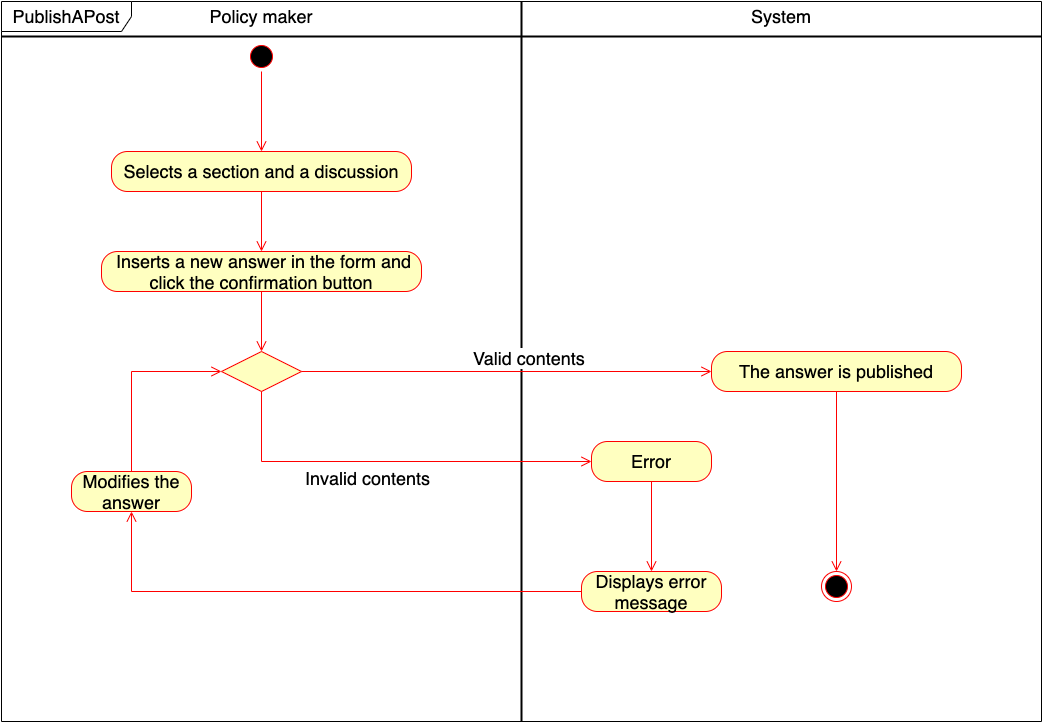
\includegraphics[scale=0.35]{images/use_cases_diagram/policymaker_publish_post.png}
        \caption{Publish a post by Policy maker}
        \label{fig:policymaker_publish_post}
    \end{figure}
\FloatBarrier

\newpage

    \begin{longtable}{p{.25\textwidth} | p{.75\textwidth}}
        \caption{Modify a post by Policy maker}
    \label{tab:pm_modify_post}\\
        \hline
        \textbf{ID} & 12\\
        \hline
        \textbf{Name}  &  Modify a post by Policy maker\\
        \hline
        \textbf{Actor}  &  Policy maker\\
        \hline
        \textbf{Entry condition}  &  \begin{itemize}
            \item  The Policy maker is already registered in the system
            \item  The Policy maker is already logged in the system
            \item  The Policy maker is in the discussion page where the post is present
        \end{itemize}\\
        \hline
        \textbf{Input} & Post\\
        \hline
        \textbf{Events flow} & \begin{itemize}
                \item The Policy maker press on the “Modify” button on the selected post
                \item The System returns to the Policy maker the edit page
                \item The Policy maker introduces the changes in the post
                \item The Policy maker confirms the changes by clicking the confirmation button
                \end{itemize}
                 \\
        \hline
        \textbf{Exit condition} & The changes are introduced in the post\\
        \hline
        \textbf{Exception} & The Policy maker tries to insert invalid contents (invalid characters, invalid file format, etc...)\\ \hline
        \textbf{Special requirements} & The Policy maker can modify every post \\ \hline
    \end{longtable}
    \begin{figure}[h!]
        \centering
        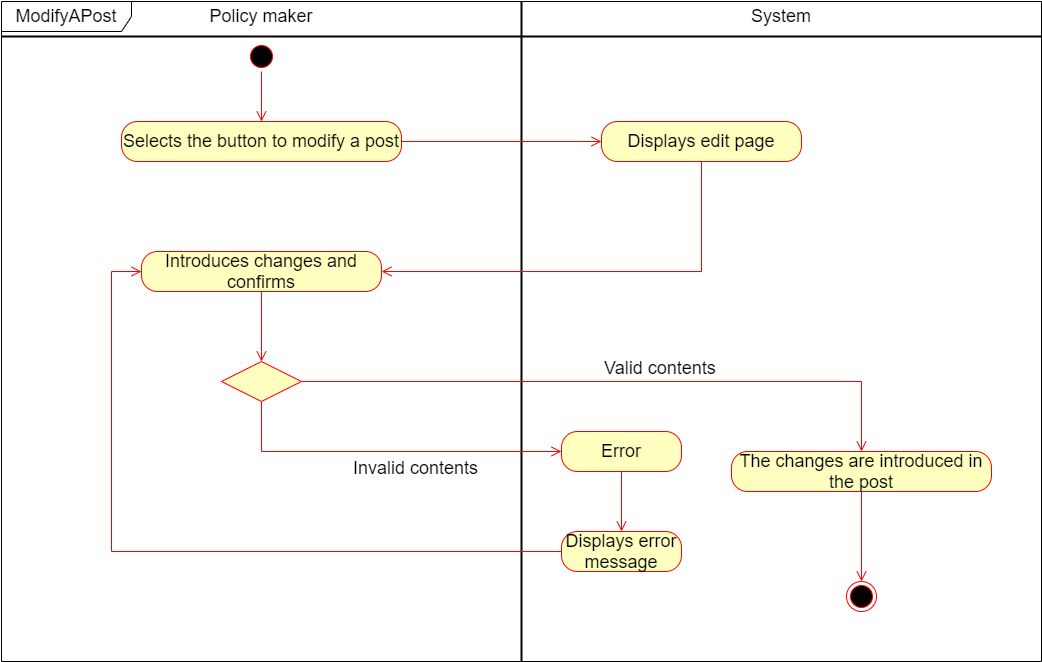
\includegraphics[scale=0.35]{images/use_cases_diagram/policymaker_modify_post.png}
        \caption{Modify a post by Policy maker}
        \label{fig:policymaker_modify_post}
    \end{figure}
    \FloatBarrier

\begin{longtable}{p{.25\textwidth} | p{.75\textwidth}}
        \caption{Delete a post by Policy maker}
    \label{tab:pm_delete_post}\\
        \hline
        \textbf{ID} & 13\\
        \hline
        \textbf{Name}  &  Delete a post by Policy maker\\
        \hline
        \textbf{Actor}  &  Policy maker\\
        \hline
        \textbf{Entry condition}  &  \begin{itemize}
            \item  The Policy maker is already registered in the system
            \item  The Policy maker is already logged in the system
            \item The post is already published
            \item  The Policy maker is in the discussion page where the post is present
        \end{itemize}\\
        \hline
        \textbf{Input} & Post\\
        \hline
        \textbf{Events flow} & \begin{itemize}
                \item The Policy maker press on the “Delete” button on the selected post
                \item The System returns to the Policy maker a confirmation message
                \item The Policy maker confirms the operation by clicking the confirmation button
                \end{itemize}
                 \\
        \hline
        \textbf{Exit condition} & The post is deleted from the forum\\
        \hline
        \textbf{Exception} & The Policy maker doesn't confirm the operation\\ \hline
        \textbf{Special requirements} & The Policy maker can delete every post\\ \hline

    \end{longtable}
    
    \begin{figure}[h!]
        \centering
        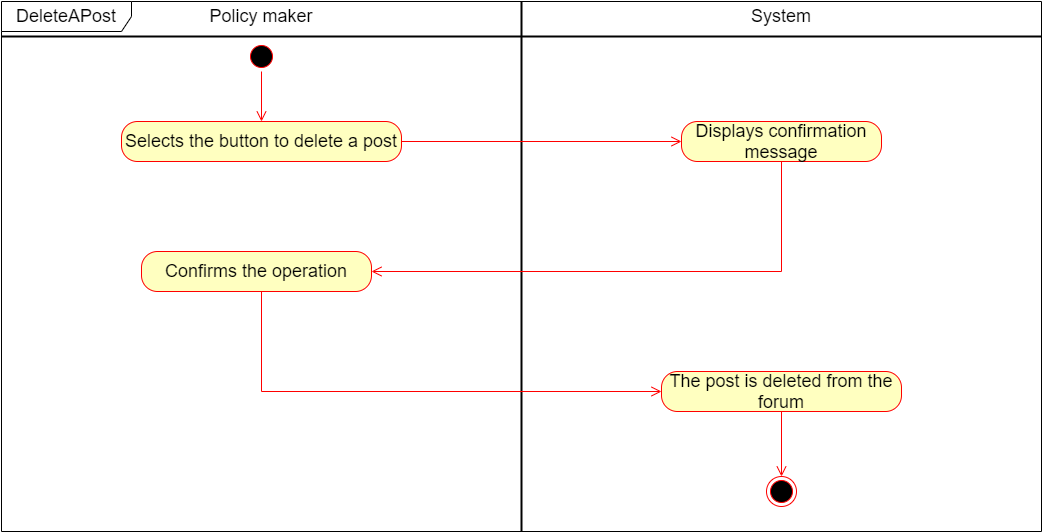
\includegraphics[scale=0.38]{images/use_cases_diagram/policymaker_delete_post.png}
        \caption{Delete a post by Policy maker}
        \label{fig:policymaker_delete_post}
    \end{figure}
    \FloatBarrier
    \newpage
    \begin{longtable}{p{.25\textwidth} | p{.75\textwidth}}
    \caption{Create a new discussion}
    \label{tab:create_new_discussion}\\
        \hline
        \textbf{ID} & 14\\
        \hline
        \textbf{Name}  &  Create a new discussion\\
        \hline
        \textbf{Actor}  &  Policy maker\\
        \hline
        \textbf{Entry condition}  &  \begin{itemize}
            \item The Policy maker is already registered in the system
            \item The Policy maker is already logged in the system
            \item The Policy maker is in the forum home page
        \end{itemize}\\
        \hline
        \textbf{Events flow} & \begin{itemize}
                \item The Policy maker selects the topic of his interest
                \item The Policy maker click on the “New discussion” button
                \item The Policy maker writes/uploads the report 
                \item The Policy maker confirms the operation by clicking on the confirmation button
                \end{itemize}
                 \\
        \hline
        \textbf{Exit condition} & The report is saved and published in the system\\
        \hline
        \textbf{Exception} & The Policy maker tries to insert invalid contents\\\hline
    
    \end{longtable}
    
    \begin{figure}[h!]
        \centering
        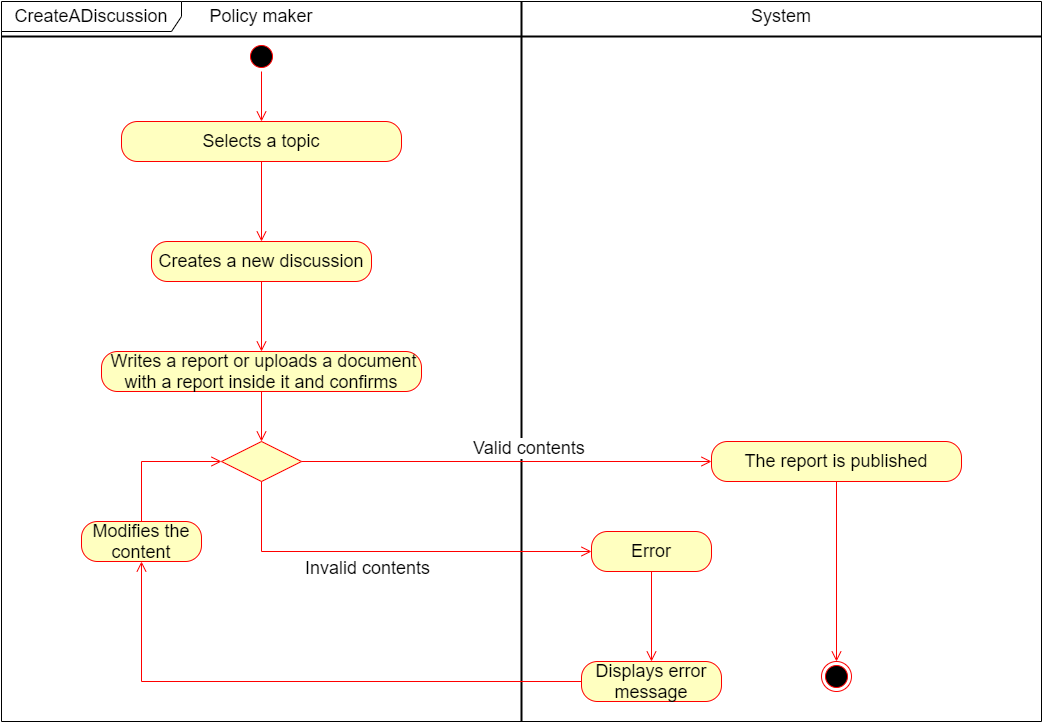
\includegraphics[scale=0.35]{images/use_cases_diagram/policymaker_create_discussion.png}
        \caption{Create a new discussion}
        \label{fig:policymaker_create_discussion}
    \end{figure}
 \FloatBarrier
 
 \begin{longtable}{p{.25\textwidth} | p{.75\textwidth}}
        \caption{Delete a discussion}
    \label{tab:pm_delete_discussion}\\
        \hline
        \textbf{ID} & 15\\
        \hline
        \textbf{Name}  &  Delete a discussion\\
        \hline
        \textbf{Actor}  &  Policy maker\\
        \hline
        \textbf{Entry condition}  &  \begin{itemize}
            \item  The Policy maker is already registered in the system
            \item  The Policy maker is already logged in the system
            \item The discussion is already existing
            \item  The Policy maker is in the topic where the discussion is present
        \end{itemize}\\
        \hline
        \textbf{Input} & Discussion\\
        \hline
        \textbf{Events flow} & \begin{itemize}
                \item The Policy maker press on the “Delete” button on the selected discussion
                \item The System returns to the Policy maker a confirmation message
                \item The Policy maker confirms the operation by clicking the confirmation button
                \end{itemize}
                 \\
        \hline
        \textbf{Exit condition} & The discussion and all the posts inside of it are deleted from the forum\\
        \hline
        \textbf{Exception} & The Policy maker doesn't confirm the operation\\ \hline
        \textbf{Special requirements} & The Policy maker can delete every discussion\\ \hline

    \end{longtable}
    
    \begin{figure}[h!]
        \centering
        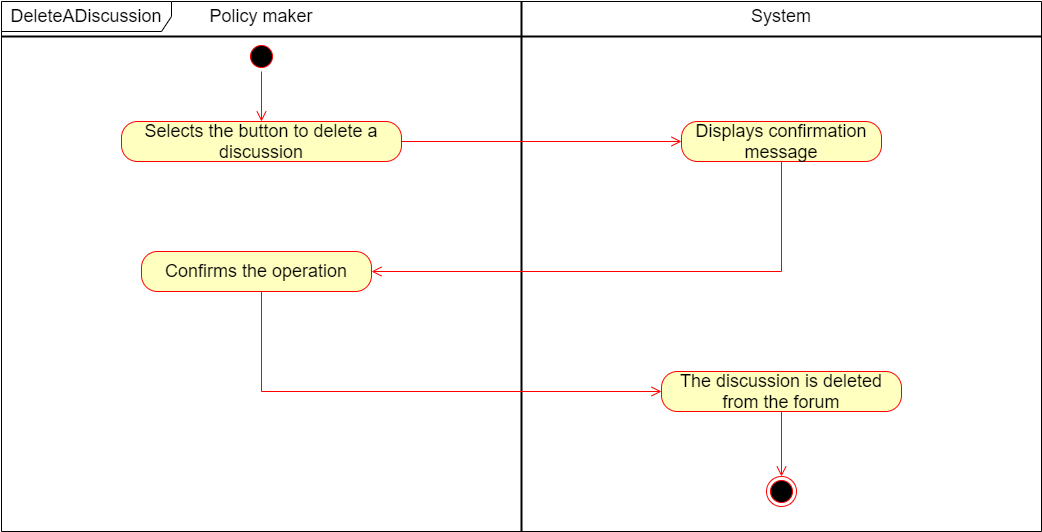
\includegraphics[scale=0.38]{images/use_cases_diagram/policymaker_delete_discussion.png}
        \caption{Delete a discussion}
        \label{fig:policymaker_delete_discussion}
    \end{figure}
    \FloatBarrier
    \newpage
    \begin{longtable}{p{.25\textwidth} | p{.75\textwidth}}
     \caption{Confirm pending post}
        \label{tab:Confirm_pending_post}\\
        \hline
        \textbf{ID} & 16\\
        \hline
        \textbf{Name}  &  Confirm pending post\\
        \hline
        \textbf{Actor}  &  Policy maker\\
        \hline
        \textbf{Entry condition}  &  
        \begin{itemize}
                \item The Policy maker is already registered in the system
                \item The Policy maker is already logged in the system
                \item The Policy maker is in the forum home page
         \end{itemize}\\
        \hline
        \textbf{Events flow} & 
        \begin{itemize}
                \item The Policy maker selects the “Moderator Area” button
                \item The system displays the Moderator Area
                \item The Policy maker selects the “pending list” option
                \item The system displays the pending post list
                \item The Policy maker selects a pending post request
                \item The system displays the selected post
                \item The Policy maker reviews the post
                \item The Policy maker approves the post by clicking on the confirmation button
                 \end{itemize}
                 \\
        \hline
        \textbf{Exit condition} &
        \begin{itemize}
                \item The post is removed from the pending list and published in the forum
                \item A notification is sent to the Author of the post
                \end{itemize}
                \\
        \hline
        \textbf{Special Requirements} & The pending post must be accepted no later than 30 days after it is sent by User\\
        \hline
       
       
    \end{longtable}
    

    \begin{longtable}{p{.25\textwidth} | p{.75\textwidth}}
     \caption{Decline pending post}
    \label{tab:decline_pending_post}\\
        \hline
        \textbf{ID} & 17\\
        \hline
        \textbf{Name}  &  Decline pending post\\
        \hline
        \textbf{Actor}  &  Policy maker\\
        \hline
        \textbf{Entry condition}  &  \begin{itemize}
            \item The Policy maker is already registered in the system
            \item The Policy maker is already logged in the system
            \item The Policy maker is in the forum home page

        \end{itemize}\\
        \hline
        \textbf{Events flow} & \begin{itemize}
                \item The Policy maker selects the “Moderator Area” button
                \item The system displays the Moderator Area
                \item The Policy maker selects the “pending list” option 
                \item The system displays the pending post list
                \item The Policy maker selects a pending post request
                \item The Policy maker reviews the post
                \item The Policy maker declines the approval of the post by clicking on the decline button
                \end{itemize}
                 \\
        \hline
        \textbf{Exit condition} & \begin{itemize}
            \item The pending post request is deleted and removed from the pending post list
            \item A notification is sent to the Author of the post
        \end{itemize}\\
        \hline
   
    \end{longtable}
\begin{figure}[h!]
        \centering
        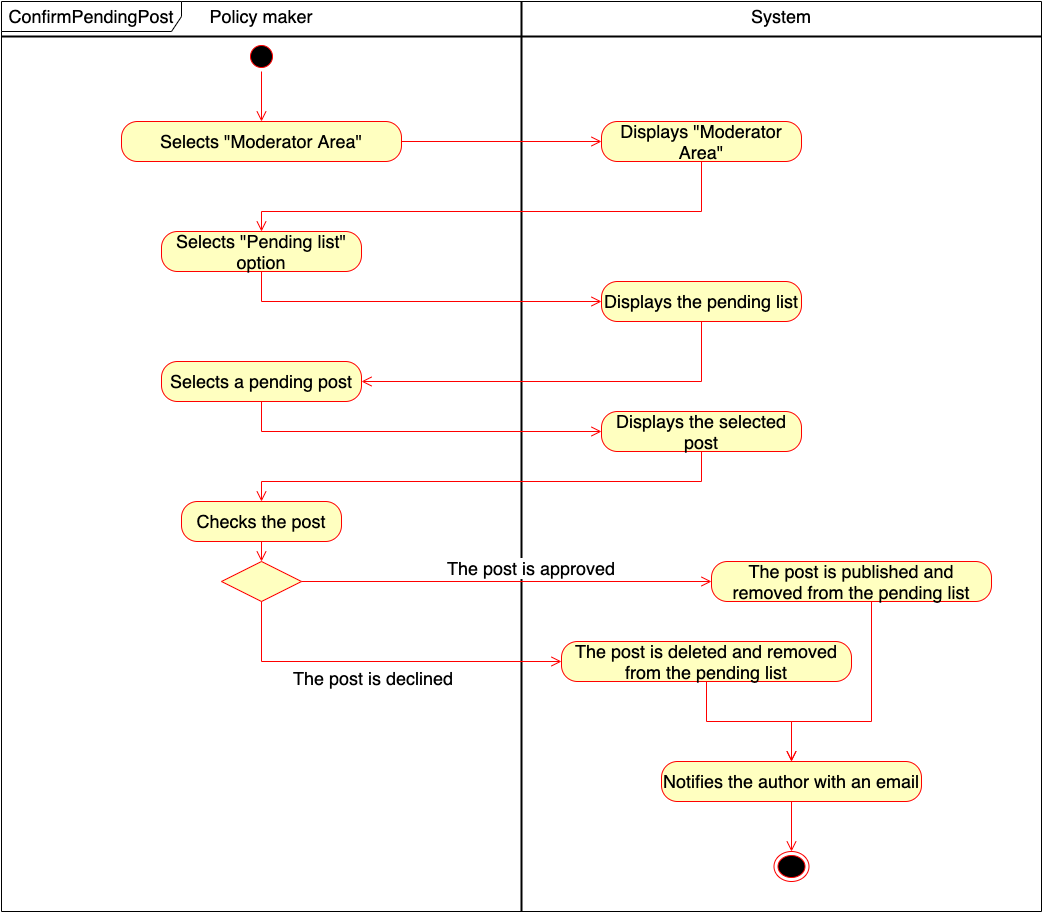
\includegraphics[scale=0.35]{images/use_cases_diagram/policymaker_pending_post.png}
        \caption{Confirm or decline a pending post}
        \label{fig:policymaker_pending_post}
    \end{figure}
\FloatBarrier
    
    \newpage
    
          \begin{longtable}{p{.25\textwidth} | p{.75\textwidth}}
          \caption{Recalculate new deviance}
    \label{tab:recalculate_new_deviance}\\
        \hline
        \textbf{ID} & 18\\
        \hline
        \textbf{Name}  &  Recalculate new Deviance\\
        \hline
        \textbf{Actor}  &  Policy maker\\
        \hline
        \textbf{Entry condition}  &  \begin{itemize}
            \item The Policy maker is already registered in the system
            \item The Policy maker is already logged in the system
            \item The Policy maker is in the home page
        \end{itemize}\\
        \hline
        \textbf{Input} & Parameters and data\\
        \hline
        \textbf{Events flow} & \begin{itemize}
                \item The Policy maker selects the “Reserved Area” button
                \item The System displays the Reserved Area
                \item The Policy maker selects the “Deviance” option
                \item The System displays the actual Deviance, calculated by default by the system, and a list of parameters that he can select in order to recalculate a custom Deviance
                \item The Policy maker selects different parameters
                \item The Policy maker clicks on Recalculate
                \item The System recalculate the new Deviance
                \item The System displays the new ranking list

                \end{itemize}
                 \\
        \hline
        \textbf{Exit condition} & The Deviance is recalculated and it's displayed the new ranking list\\
        \hline
        \textbf{Exception} & The Policy maker didn’t selects any parameter\\ \hline
        
    
    \end{longtable}
    
    \begin{figure}[h!]
        \centering
        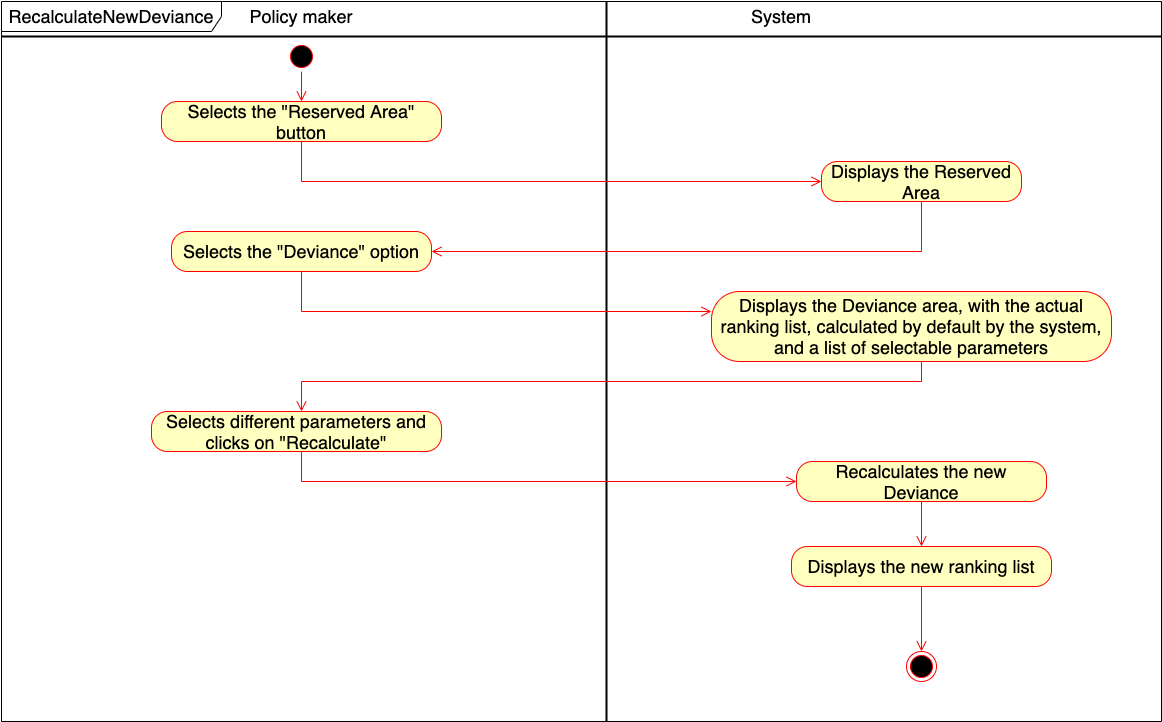
\includegraphics[scale=0.35]{images/use_cases_diagram/policymaker_recalculate_deviance.png}
        \caption{Recalculate new deviance}
        \label{fig:policymaker_recalculate_deviance}
    \end{figure}
    \FloatBarrier
